\documentclass[preview=true, border=10pt]{standalone}

\usepackage[compat=1.1.0]{tikz-feynman}

\newcommand{\BdbarToDpiPenguinSize}{6.4}

\begin{document}
	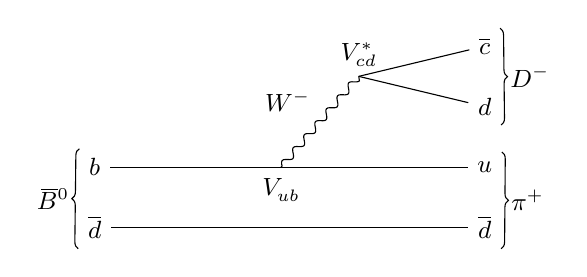
\begin{tikzpicture}
		\begin{feynman}
			\vertex (a1) {\small$b$};
			\vertex[right=\BdbarToDpiPenguinSize*0.37 cm of a1] (a2);
			\vertex[right=\BdbarToDpiPenguinSize*0.37 cm of a2] (a3) {\small$u$};
			\vertex[below=\BdbarToDpiPenguinSize*0.12 cm of a1] (b1) {\small$\overline d$};
			\vertex[below=\BdbarToDpiPenguinSize*0.12 cm of a3] (b2) {\small$\overline d$};
			\vertex[above=\BdbarToDpiPenguinSize*0.12 cm of a3] (c1) {\small$d$};
			\vertex[above=\BdbarToDpiPenguinSize*0.12 cm of c1] (c3) {\small$\overline c$};
			\vertex at ($(c1)!0.5!(c3) - (\BdbarToDpiPenguinSize*0.25 cm, 0)$) (c2);
			\diagram* {
			(a3) -- [plain] (a2) -- [plain] (a1),
			(b1) -- [plain] (b2),
			(c3) -- [plain] (c2) -- [plain] (c1),
			(a2) -- [boson, edge label={\small$W^{-}$}] (c2),
			};
			\draw [decoration={brace}, decorate] (b1.south west) -- (a1.north west) node [pos=0.5, left] {\small$\kern 0.18em\overline{\kern -0.18em B}{}^{0}$};
			\draw [decoration={brace}, decorate] (a3.north east) -- (b2.south east) node [pos=0.5, right] {\small$\pi^{+}$};
			\draw [decoration={brace}, decorate] (c3.north east) -- (c1.south east) node [pos=0.5, right] {\small$D^{-}$};

			\vertex [below=\BdbarToDpiPenguinSize*0.001 cm of a2] {\small$V_{ub}^{\phantom{\ast}}$};
			\vertex [above=\BdbarToDpiPenguinSize*0.001 cm of c2] {\small$V_{cd}^{\ast}$};
		\end{feynman}
	\end{tikzpicture}
\end{document}
